\documentclass{beamer}
\setbeamertemplate{caption}[numbered]
\usepackage{graphicx}
\usepackage{svg}
\usepackage[utf8]{inputenc}
\usepackage[english]{babel}
\graphicspath{{Graphs/}}
\usepackage{comment}
\usepackage{verbatim}
\usepackage{hyperref}
\mode<presentation>
{
	\usetheme{AnnArbor}
	\usecolortheme{crane}
}

\title[Data Visualization using Stata]{Data Visualization using Stata}
\subtitle[ISRC Workshop]{Iowa Social Research Center (ISRC) Workshop}
\author[Wallace]{Desmond D. Wallace}
\institute[University of Iowa]{Department of Political Science\\The University of Iowa\\Iowa City, IA}

\date{November 10, 2017}

\begin{document}
	
\begin{frame}
	\titlepage
\end{frame}

\section{Introduction}

\begin{frame}
	\frametitle{Why Visualize Data?}
		\begin{itemize}
			\item One can communicate information clearly and effectively via graphics
			\item Effective data visuals helps users analyze and reason with data
			\item Make complex data accessible, understandable and usable
			\item Display patterns and/or relationships in one's dataset
			\item One can visualize patterns and/or relationships with respect to discrete and/or continuous variables
		\end{itemize}
\end{frame}

\section{Univariate Graphs}
\subsection{Graph Types}

\begin{frame}
	\frametitle{\texttt{graph \textit{type}} -- Available Types}
		\begin{itemize}
			\item Bar Graphs
			\item Box Plots
			\item Distribution Graphs
				\begin{itemize}
					\item Histograms
					\item Kernel Density Estimation Plots
				\end{itemize}
			\item Dot Charts (Not Covered)
			\item Pie Charts (Not Covered)
		\end{itemize}
\end{frame}

\subsection{Bar Graphs}

\begin{frame}
	\frametitle{Introduction}
		\begin{itemize}
			\item Constructs bars used to visualize the distribution of a categorical variable
			\item Similar to a histogram
			\item Default is to construct a bar for each variable level
		\end{itemize}
\end{frame}

\begin{frame}
	\frametitle{Syntax}
		\begin{itemize}
			\item Basic: \texttt{graph bar (\textit{stat}) \textit{yvars}}, where \textit{yvars} is a variable list
			\item Displays specified summary statistic for variable(s); default is the mean
			\item Other statistics include the median, count, various percentiles, etc.
			\item Can specify multiple (\textit{stat}) \textit{yvars}
			\item Can display summary statistic of specified variable based on levels of a categorical variable via the \texttt{over(\textit{varname})} option
			\item Advanced: \texttt{graph bar (\textit{stat}) \textit{yvars}, over(\textit{varname})}
		\end{itemize}
\end{frame}

\begin{frame}
	\frametitle{Syntax}
		\begin{itemize}
			\item \textit{yvars} is optional when \texttt{over(\textit{varname})} is specified (Stata 14 only)
			\item Acceptable syntax: \texttt{graph bar, over(\textit{varname})}
			\item Percentage is now treated as default statistic, calculated based on levels of \textit{varname}
			\item Can change the statistic to \texttt{count}, which reports the frequency totals for each level of \textit{varname}
			\item Replace \texttt{bar} with \texttt{hbar} to produce horizontal bar graph.
			\item See \texttt{help graph bar} for additional information
		\end{itemize}
\end{frame}

\begin{frame}
	\frametitle{Bar Graph Example -- PDF}
		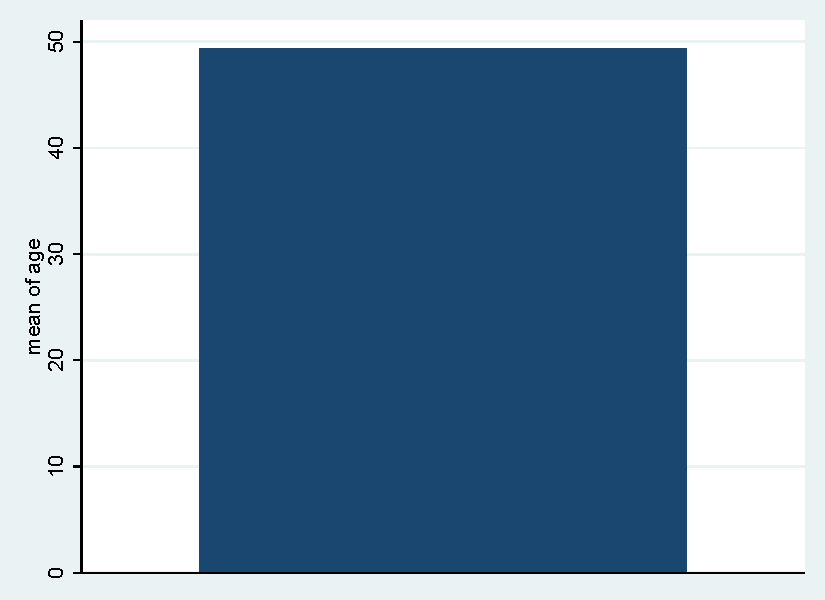
\includegraphics[scale=0.7]{DVgraph01.pdf}
\end{frame}

\begin{frame}
	\frametitle{Bar Graph Example -- PNG}
		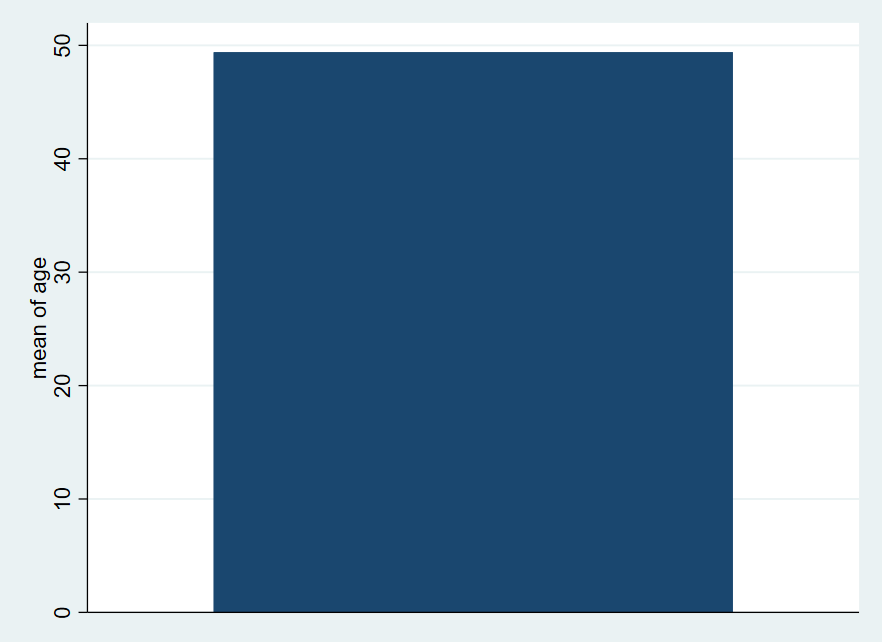
\includegraphics[scale=0.3]{DVgraph01.png}
\end{frame}

\subsection{Box Plots}

\begin{frame}
	\frametitle{Introduction}
		\begin{itemize}
			\item Displays a box and ``whiskers'' that visualizes the distribution of a continuous variable
			\item Box
				\begin{itemize}
					\item Bordered at the 25th and 75th percentiles (Q1 and Q3)
					\item An additional \textit{median} line at the 50th percentile
				\end{itemize}
			\item ``Whiskers''
				\begin{itemize}
					\item Lower Adjacent Value (LAV) -- Smallest observation greater than or equal to the lower inner fence (LIF), which is $\mbox{Q1}-1.5\times \mbox{IQR}$, where $\mbox{IQR}=\mbox{Q3}-\mbox{Q1}$
					\item Upper Adjacent Value (UAV) -- Largest observation smaller than or equal to the upper inner fence (UIF), which is $\mbox{Q3}+1.5\times \mbox{IQR}$
				\end{itemize}
			\item Any observation falling smaller (larger) than the adjacent values appears as dots
		\end{itemize}
\end{frame}

\begin{frame}
	\frametitle{Syntax}
		\begin{itemize}
			\item Basic: \texttt{graph box \textit{yvars}}, where \textit{yvars} is a variable list
			\item Can display box plots of specified variable(s) based on levels of a categorical variable via the \texttt{over(\textit{varname})} option
			\item Advanced: \texttt{graph box \textit{yvars}, over(\textit{varname})}
			\item Replace \texttt{box} with \texttt{hbox} to produce horizontal box plot(s).
			\item See \texttt{help graph box} for additional information
		\end{itemize}
\end{frame}

\subsection{Distribution Plots}

\begin{frame}
	\frametitle{Histograms}
		\begin{itemize}
			\item A graph that shows the distribution of a variable that takes on many values (Acock 2014).
			\item Syntax: \texttt{\underline{hist}ogram \textit{varname}, \textit{options}}
			\item Can be used for both discrete and continuous variables
			\item Use the command \texttt{help \underline{hist}ogram} for more information
		\end{itemize}
\end{frame}

\begin{frame}
	\frametitle{Kernel Density Estimation Plots}
		\begin{itemize}
			\item Non-parametric method for estimating the PDF (PMF) of a random variable.
			\item Syntax: \texttt{kdensity \textit{varname}, \textit{options}}
			\item Can be used for both discrete and continuous variables
			\item Use the command \texttt{help kdensity} for more information
		\end{itemize}
\end{frame}

\section{Bivariate Graphs}
\subsection{Introduction}

\begin{frame}
	\frametitle{Introduction}
		\begin{itemize}
			\item Used to display relationships between two numeric-type variables
			\item Represents over 30 different types of graphs, which can be grouped into multiple categories
			\item Easy to overlay \texttt{twoway}-type plots
				\begin{itemize}
					\item Enclose graph type and variables in parentheses $()$
					\item Separate graphs via double vertical bars $||$
				\end{itemize}
		\end{itemize}
\end{frame}

\begin{frame}
	\frametitle{Available Types Not Covered}
		\begin{itemize}
			\item Area Plots
			\item Bar Plots
			\item Range Plots*
			\item Regression Fits and Confidence Intervals*
			\item Functions*
			\item Contour Plots
		\end{itemize}
\end{frame}

\begin{frame}
	\frametitle{Available Types Covered}
		\begin{itemize}
			\item Scatterplots
			\item Line Plots
			\item Distribution Plots
				\begin{itemize}
					\item Histogram
					\item Kernel Density Plot
				\end{itemize}
		\end{itemize}
\end{frame}

\subsection{Scatterplots}

\begin{frame}
	\frametitle{Introduction}
		\begin{itemize}
			\item Utilize horizontal and vertical axes to plot data
			\item Communicates how much one variable is affected by another
			\item Visual representation of the correlation between two variables
		\end{itemize}
\end{frame}

\begin{frame}
	\frametitle{Syntax}
		\begin{itemize}
			\item Basic: \texttt{scatter \textit{varlist}}, where \textit{varlist} is a variable list
			\item At least two variables need to be specified; last variable specified is treated as ``independent'' variable (located on the $x$-axis).
			\item Can generate scatterplots based on levels of a categorical variable via the \texttt{by(\textit{varname})} option
			\item Advanced: \texttt{scatter \textit{varlist}, by(\textit{varname})}
			\item See \texttt{help scatter} for additional information
		\end{itemize}
\end{frame}

\begin{frame}
	\frametitle{Scatterplot Example -- PDF}
		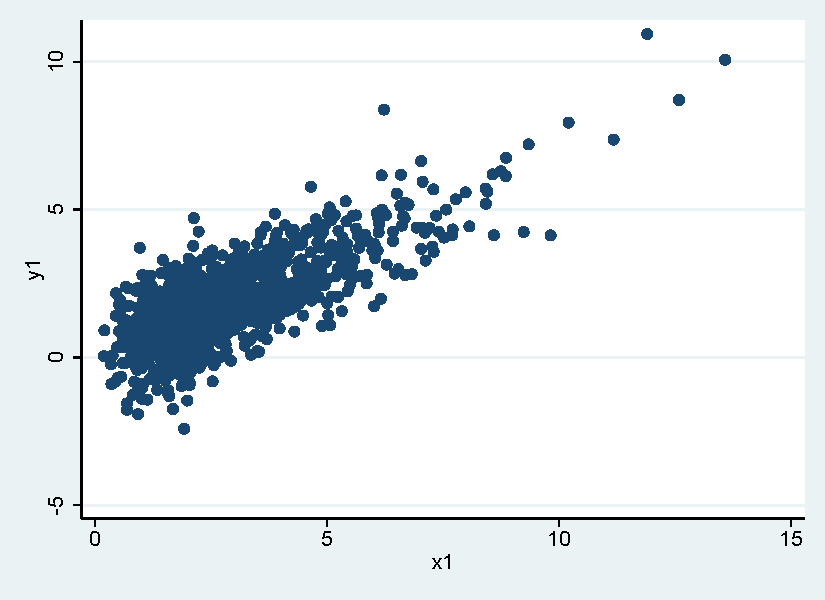
\includegraphics[scale=0.7]{DVgraph02a.pdf}
\end{frame}

\begin{frame}
	\frametitle{Scatterplot Example -- PNG}
		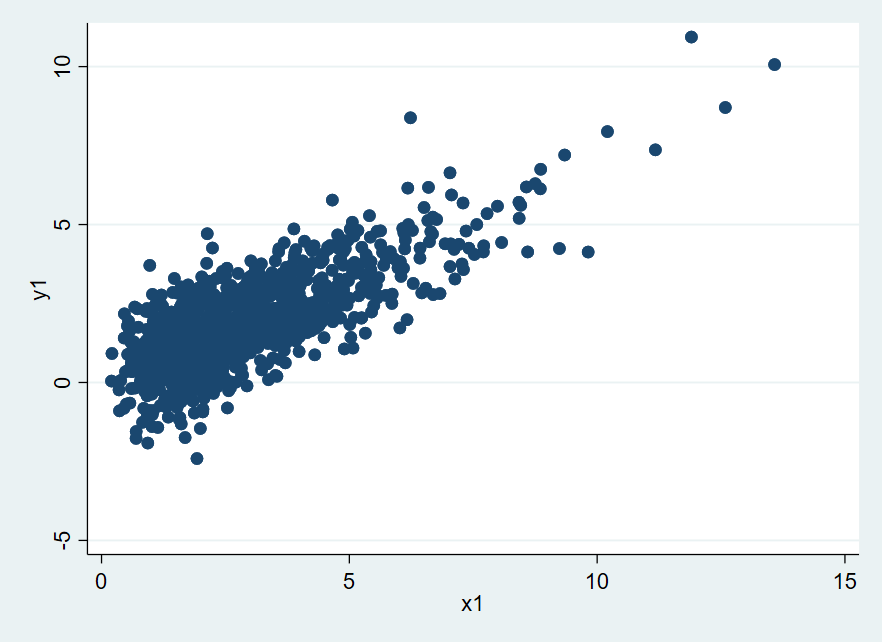
\includegraphics[scale=0.3]{DVgraph02a.png}
\end{frame}

\subsection{Line Plots}

\begin{frame}
	\frametitle{Introduction}
		\begin{itemize}
			\item Shows frequency of data along a number line
			\item Similar to a scatterplot, except the points are connected
			\item Visual representation of a variable's trend
		\end{itemize}
\end{frame}

\begin{frame}
	\frametitle{Syntax}
		\begin{itemize}
			\item Basic: \texttt{twoway line \textit{varlist}}, where \textit{varlist} is a variable list
			\item At least two variables need to be specified; last variable specified is treated as ``independent'' variable (located on the $x$-axis).
			\item The default is to construct the graph based on the ordering of the dataset
			\item Either sort the dataset using the \texttt{sort} command, or use the \texttt{sort} option along with the \texttt{twoway line} command
			\item See \texttt{help twoway line} for additional information
		\end{itemize}
\end{frame}

\subsection{Histograms and Kernel Density}

\begin{frame}
	\frametitle{\texttt{twoway} Version}
		\begin{itemize}
			\item Same as \texttt{hist} and \texttt{kdensity}, except
				\begin{itemize}
					\item Allows overlaying of a normal density or a kernel estimate of the density
					\item If a density estimate is overlaid, it scales the density to reflect the scaling of the bars
				\end{itemize}
			\item Basic Syntax
				\begin{itemize}
					\item Histogram: \texttt{twoway histogram \textit{varname}}
					\item Kernel Density: \texttt{twoway kdensity \textit{varname}}
				\end{itemize}
			\item See \texttt{help histogram} and \texttt{help kdensity} for additional information
		\end{itemize}
\end{frame}

\section{Editing Graphs}

\begin{frame}
	\frametitle{Graph Editor vs. Commands}
		\begin{itemize}
			\item Two ways to edit Stata graphs: commands and the Graph editor
			\item Whenever possible, best to use commands to make changes to your graphs
			\item Situations can arise, however, where the graph editor is better suited than using the commands (e.g. adding objects, modifying objects)
			\item Changes made via the graph editor can be recorded, and applied to future graphs
			\item See \textit{A Visual Guide to Stata Graphics, Third Edition}, pages 82-88, for a more detailed discussion
		\end{itemize}
\end{frame}

\section{New Features in Stata 15}
\subsection{SVG Export}

\begin{frame}
	\frametitle{Scalable Vector Graphics (SVG)}
		\begin{itemize}
			\item SVG images are scalable without image quality loss
			\item Used on webpages and EPUB ebook documents
			\item Compatible with modern desktop and mobile web browsers
			\item Editable with vector graphics applications and text editors (e.g. Adobe Illustrator)
		\end{itemize}
\end{frame}

\subsection{Transparency}

\begin{frame}
	\frametitle{Graph Transparency}
		\begin{itemize}
			\item Adjust color transparency in almost every element of a Stata graph
			\item Change percentage of opacity (Default: 100\% opaque)
			\item See aspects of your data that weren't visible before
			\item Print graphs with transparency or export them to PDF, SVG, PNG, TIFF, or EMF
			\item NOTE: Only applicable in \texttt{twoway} graphs
		\end{itemize}
\end{frame}

\begin{frame}
	\frametitle{Transparency Example -- PDF}
		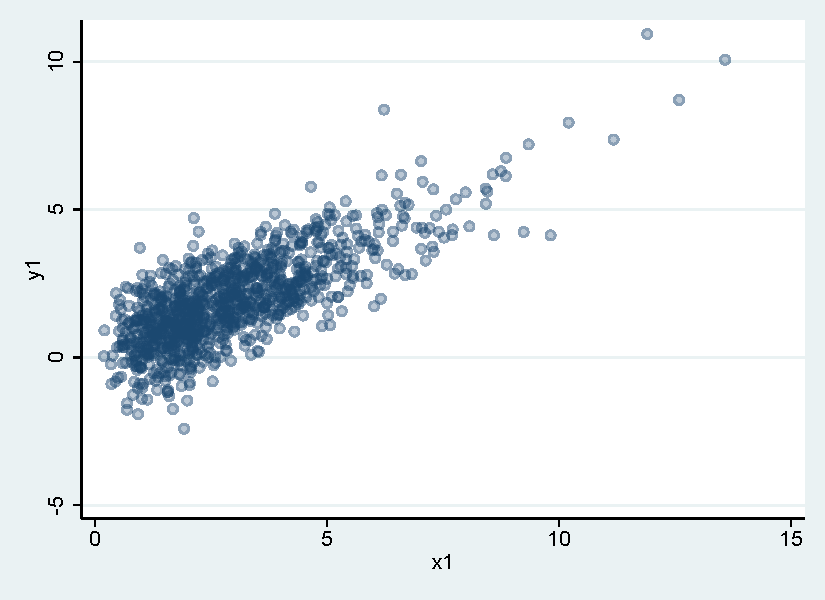
\includegraphics[scale=0.7]{DVgraph02b.pdf}
\end{frame}

\begin{frame}
	\frametitle{Transparency Example -- PNG}
		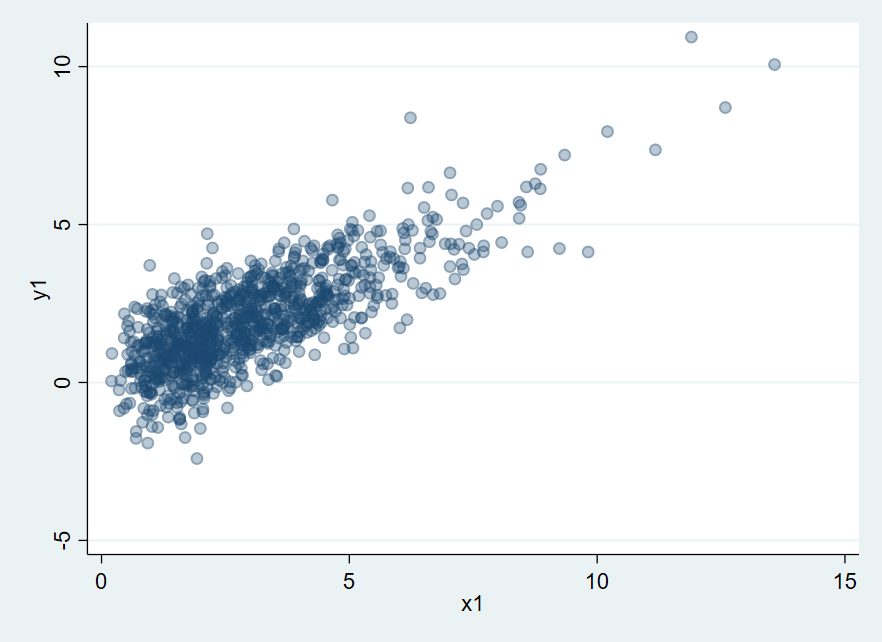
\includegraphics[scale=0.3]{DVgraph02b.png}
\end{frame}

\begin{frame}
	\begin{center}
		\begin{LARGE}
			Email: desmond-wallace@uiowa.edu\\
			Any Questions?
		\end{LARGE}
	\end{center}
\end{frame}

\end{document}
